\section{Network Architecture}\label{sec:Network_Architecture}
\begin{definition}[Network Architecture]\label{def:Network_Architecture}
  \emph{Network Architecture} is:
  \begin{itemize}[noitemsep]
  \item How the overall system is designed: what components there are and how they interact.
  \item Protocols and technologies for all the layers of the network stack.
  \item Physical infrastructure: base stations, cables, antennas, routers, etc.
  \item How everything works together to meet the overall performance goals for the whole system.
  \end{itemize}
\end{definition}

\subsection{Wireless vs. Wired Networks}\label{subsec:Wireless_vs_Wired}
Wireless and wired (fixed) networks operate under the same underlying network principles.
However, wireless systems have a very different set of challenges to also contend with, because of the nature of wireless radio communication, and it being a broadcast medium.

The biggest problems for wireless networks that wired networks do not have are:
\begin{itemize}[noitemsep]
\item Interference, \Cref{subsec:Wireless_Interference}
\item Mobility, \Cref{subsec:Wireless_Mobility}
\item Wireless channels:
  \begin{itemize}[noitemsep]
  \item Path loss
  \item Shadowing
  \item Fading
  \item These will not be handled in this course.
  \end{itemize}
\end{itemize}

\subsection{Interference in Wireless Networks}\label{subsec:Wireless_Interference}
The biggest difference between wired and wireless networks when it comes to interference is because of the transportation medium.
In a wired system, discrete connections form isolated links between nodes.
The properties of any single link do not directly affect the properties of any other node.

However, in wireless networks, each of the nodes is broadcasting into space.
Any of these nodes' broadcasts can affect any of the other nodes.
You can think of it as if each node has a large sphere extending radially outwards, where multiple nodes can cover the same zone.
Additionally, this may also mean that some nodes are dependent on other nodes.

\subsubsection{Performance in Interfering Networks}\label{subsubsec:Performance_Interfering_Networks}
In the work done by \citeauthor{Wireless_Network_Capacity}, it was found there is a closed-form solution for the performance of interfering wireless networks.

Place $n$ nodes on a unit disk.
Each node as the capacity $W$ bits per second.
Then, the upper bound on the capacity for the network as $n \rightarrow \infty$ is
\begin{equation}\label{eq:Wireless_Network_Capacity_Upper_Bound}
  \frac{W}{\sqrt{n \log(n)}}
\end{equation}

If the nodes are placed optimally, i.e.\ each node is placed such that its transmission range never crosses another node's range.
Then the capacity of the network is given in \Cref{eq:Wireless_Network_Capacity_Optimal}
\begin{equation}\label{eq:Wireless_Network_Capacity_Optimal}
  \frac{W}{\sqrt{n}}
\end{equation}

%%% Local Variables:
%%% mode: latex
%%% TeX-master: "../../ETSN10-Network_Architecture_Performance-Reference_Sheet"
%%% End:


\subsection{Mobility}\label{subsec:Wireless_Mobility}
\begin{definition}[Mobility]\label{def:Mobility}
  \emph{Mobility} is a unique property of wireless networks.
  Since the nodes are not fixed in place by anything, they are free to roam/move.
  This is a big problem, because nodes can enter, leave, and move freely throughout/through the network.
\end{definition}

There are 3 classifications of mobility.
\begin{enumerate}[noitemsep]
\item Pedestrian: $\approx 1.5 \si{\meter/\second}$
\item Vehicle: $5-33 \si{\meter/second}$
\item High-Speed: $> 70 \si{\meter/\second}$
\end{enumerate}

\nameref{def:Mobility} has several effects on a wireless network system.
\begin{enumerate}[noitemsep]
\item Physical Layer
  \begin{itemize}[noitemsep]
  \item Doppler shift
  \item Constantly changing channel $\rightarrow$ higher bit-error rate
  \end{itemize}

\item Data-Link Layer/MAC
  \begin{itemize}[noitemsep]
  \item Which nodes share “links” (and thus can experience collisions) constantly changes.
  \item \nameref{def:Hidden_Node} and \nameref{def:Exposed_Node} problems!
  \end{itemize}

\item Network Layer
  \begin{itemize}[noitemsep]
  \item Constantly changing topology $\rightarrow$ need to constantly change end-to-end path through the network.
  \end{itemize}

\item Transport/Application Layers
  \begin{itemize}[noitemsep]
  \item Not directly affected.
  \item Delays and errors at lower layers can cause problems though.
  \end{itemize}
\end{enumerate}

%%% Local Variables:
%%% mode: latex
%%% TeX-master: "../../ETSN10-Network_Architecture_Performance-Reference_Sheet"
%%% End:


\subsection{Licensed vs. Unlicensed Spectrum}\label{subsec:Licensed_vs_Unlicensed}
There are 2 types of frequencies in use by people and companies today.
\begin{enumerate}[noitemsep]
\item \nameref{subsubsec:Licensed_Spectrum}
\item \nameref{subsubsec:Unlicensed_Spectrum}
\end{enumerate}

\subsubsection{Licensed Spectrum}\label{subsubsec:Licensed_Spectrum}
The licensed spectrum requires that users obtain exclusive rights to use that frequency spectrum.
\begin{itemize}[noitemsep]
\item Solution for QoS-sensitive applications
\item Exclusive right to spectrum use
\item Network engineering possible
  \begin{itemize}[noitemsep]
  \item Predictability
  \item Manageability
  \end{itemize}

\item Complex and costly systems are generally built around these.
\item Typically big players take these.
\end{itemize}

\subsubsection{Unlicensed Spectrum}\label{subsubsec:Unlicensed_Spectrum}
The unlicensed spectrum does not require that users obtain exclusive rights, but they may require that only certain types of data can be used in that frequency.
\begin{itemize}[noitemsep]
\item Inherent best effort systems
\item ``Some'' QoS support possible
\item No right to use spectrum
  \begin{itemize}[noitemsep]
  \item Competition
  \item Collaboration
  \end{itemize}

\item Simple and cheap systems
\item For small/medium players
\end{itemize}

%%% Local Variables:
%%% mode: latex
%%% TeX-master: "../../ETSN10-Network_Architecture_Performance-Reference_Sheet"
%%% End:


\subsection{Data Rate vs. Range}\label{subsec:Data_Rate_vs_Range}
Higher data rates means lower tranmission range.
Higher data rates also means greater amounts of power required to transmit the message.

%%% Local Variables:
%%% mode: latex
%%% TeX-master: "../../ETSN10-Network_Architecture_Performance-Reference_Sheet"
%%% End:


\subsection{Centralized Infrastructure Networks}\label{subsec:Centralized_Infrastructure_Network}
\begin{definition}[Centralized Infrastructure Network]\label{def:Centralized_Infrastructure_Network}
  \emph{Centralized Infrastructure Networks} have some fixed nodes which have the connection to the wider Internet.
  These gateways are the ones that provide access to the Internet.
  This system works in a hierarchical structure, following a \nameref{def:Star_of_Stars} topology.
\end{definition}

\begin{definition}[Star-of-Stars]\label{def:Star_of_Stars}
  A network with a \emph{star-of-stars} topology is a hierarchical setup, where the leaf nodes in the system are the ones generating data to send.
  The next rows up may generate some data, but mainly serve as aggregators for the lower nodes in the system.
  Eventually, all connections terminate at one head star node.
\end{definition}

\subsubsection{Example Centralized Architectures}\label{subsubsec:Example_Centralized_Architectures}
\begin{enumerate}[noitemsep]
\item 802.11 a/b/g/n/ac
\begin{itemize}[noitemsep]
\item Most common WiFi network type, used in homes, shops, offices, etc.
\item 2.4 or 5 GHz bands, range $\approx 500 \si{\meter}$
\item MAC:\@ 802.11 DCF
\end{itemize}

\item 802.11 ah
  \begin{itemize}[noitemsep]
  \item WiFi for Internet of Things
  \item 800 MHz band, range $\approx 1 \si{\kilo \meter}$
  \item MAC:\@ 802.11 DCF with some modifications:
    \begin{itemize}[noitemsep]
    \item Relay nodes
    \item Target wake times
    \item Contention groups
    \end{itemize}
  \item Aimed at reducing energy usage and providing coverage to more nodes in a single network
\end{itemize}

\item LoRa
  \begin{itemize}[noitemsep]
  \item Low-Power Wide Area Network (LPWAN) for Internet of Things
  \item 800 MHz band, range 10s of km
  \item MAC:\@ ALOHA for the uplink, with receive windows for the downlink
  \end{itemize}
\end{enumerate}

\begin{remark*}
  For the above architectures, standard Internet routing (\nameref{def:Distance_Vector_Routing_Protocol} or \nameref{def:Link_State_Routing_Protocol}) is used.
  \begin{itemize}[noitemsep]
  \item Only one wireless hop, so no specialised routing is needed.
  \end{itemize}
\end{remark*}

\begin{remark*}
  Some wireless-aware protocols can be used at higher layers, e.g. Mobile IP, Wireless TCP (WTCP).
\end{remark*}

%%% Local Variables:
%%% mode: latex
%%% TeX-master: "../../ETSN10-Network_Architecture_Performance-Reference_Sheet"
%%% End:


\subsection{Infrastructure Mesh Networks}\label{subsec:Infrastructure_Mesh_Networks}

%%% Local Variables:
%%% mode: latex
%%% TeX-master: "../../ETSN10-Network_Architecture_Performance-Reference_Sheet"
%%% End:


\subsection{Ad-Hoc Networks}\label{subsec:Ad_Hoc_Networks}
\subsubsection{Uses of Ad-Hoc Networks}\label{subsubsec:Uses_Ad_Hoc_Network}
\subsubsection{Example Ad-Hoc Architectures}\label{subsubsec:Ad_Hoc_Architectures}
\subsubsection{Ad-Hoc Energy Usage}\label{subsubsec:Ad_Hoc_Architectures}

%%% Local Variables:
%%% mode: latex
%%% TeX-master: "../../ETSN10-Network_Architecture_Performance-Reference_Sheet"
%%% End:


\subsection{Mesh Network Routing}\label{subsec:Mesh_Network_Routing}
\begin{remark*}
  Most of these can be applied to both \nameref{def:Wireless_Mesh_Network}s and \nameref{def:Ad_Hoc_Network}s.
  However, some of the details relating to the problems due to \nameref{def:Mobility} will \textbf{NOT} apply to \nameref{def:Wireless_Mesh_Network}s.
\end{remark*}

\begin{itemize}[noitemsep]
\item Mobility causes paths to be unstable.
\item Using “traditional” shortest path algorithms is inefficient.
  \begin{itemize}[noitemsep]
  \item Dijkstra
  \item Bellman-Ford
  \item etc.
  \end{itemize}

\item Two main approaches:
  \begin{enumerate}[noitemsep]
  \item \textcolor{red}{Proactive}: Continuously update about topology and changes
    \begin{itemize}[noitemsep]
    \item Advantage: Low latency
    \item Disadvantage: Costly updates
    \end{itemize}
  \item \textcolor{red}{Reactive}: Only determine routing path when sending data
    \begin{itemize}[noitemsep]
    \item Advantage: No constant overhead
    \item Disadvantage: Delay due to route discovery
    \end{itemize}
  \end{enumerate}

\item Some hybrid protocols exist as well, which combine proactive
  and reactive approaches in different ways.
\end{itemize}

Because shortest-path routing algorithms are not usable in \nameref{def:Ad_Hoc_Network}s, what can we use?
We can route based on:
\begin{itemize}[noitemsep]
\item Interference
\item Social Similarity
\item Location
\item Residual Energy
\item Energy Usage
  \begin{itemize}[noitemsep]
  \item Multiple hops using little power vs.\@ single high power transmission.
  \end{itemize}
\end{itemize}

\subsubsection{Ad-Hoc On-Demand Distance Vector Routing}\label{subsubsec:ADOV_Routing}
\begin{definition}[Ad-Hoc On-Demand Distance Vector Routing]\label{def:ADOV_Routing}
  In \emph{Ad-hoc On-demand Distance Vector routing} (\emph{ADOV}), the sender broadcasts a ``Route Request'' packet, which is flooded throughout the whole network, until it reaches the intended receiver node.
  Each node maintains a route cache, which uses the node sequence the route request packet has gone through so far.
  Once the end node has been reached, the correct route state in each node is used to construct the link route.

  This only reacts when routes fail.
  When they do fail, the nodes go through a 2-step process.
  \begin{enumerate}[noitemsep]
  \item Attempt local recovery.
    \begin{itemize}[noitemsep]
    \item Nodes monitor neighbors
    \item Issue error message on detected problem.
    \end{itemize}
  \item If local recovery fails, the original sender repeats the route discovery process by sending another ``Route Request'' packet.
  \end{enumerate}

  The cost of this routing protocol is directly related to the rate of \nameref{def:Mobility} in the network.
  It realy only works for smaller networks with limited \nameref{def:Mobility}.

  It is currently popular in deployed systems.
\end{definition}

\subsubsection{Geographic Routing}\label{subsubsec:Geographic_Routing}
\begin{definition}[Geographic Routing]\label{def:Geographic_Routing}
  \emph{Geographics Routing} is based on the nodes’ \textbf{physical positions}, rather than network addresses or routing tables.
  Once the physically shortest route has been found, messages are then routed towards a destination location.
\end{definition}

However, \nameref{def:Geographic_Routing} has some issues as well.
\begin{itemize}[noitemsep]
\item Route discovery is costly in terms of time and energy.
\item Routing tables quickly become out of date in highly mobile
  networks.
\item Addressing a message to a position may be more useful than
  to a network address.
  \begin{itemize}[noitemsep]
  \item Sending an accident or traffic jam notification to upstream vehicles in a VANET
  \item Sending a request to collect sensor data in a particular region in a WSN
  \item Tracking something through a WSN (e.g.\@ an animal)
  \end{itemize}
\end{itemize}

To make \nameref{def:Geographic_Routing} less costly, we use \nameref{def:Localization}.
\begin{definition}[Localization]\label{def:Localization}
  In \emph{localization}, we find out where each of the nodes are in physical space.
  We can find the absolute locality with GPS, IMU, and many others.
  If we can use the relative locality, then we can use trilateration.
  This is done by having each node broadcast a signal and having each node listen for the same kind of signal.
  This signal is used to locate other beacons by using TDOA.\@
\end{definition}

\subsubsection{Greedy Forwarding}\label{subsubsec:Greedy_Forwarding}
\begin{definition}[Greedy Forwarding]\label{def:Greedy_Forwarding}
  In \emph{greedy forwarding}, we forward this packet to the node \textbf{physically closest} to the destination node.
  This guaranteed there will be no loops in the traversal of the network graph.

  There are various forms and definitions of what ``closest'' means:
  \begin{itemize}[noitemsep]
  \item Distance to target
  \item Distance along the source-destination line
  \item Smallest angle to destination (compass routing)
  \end{itemize}

  \begin{remark}[Greedy Forwarding Failure]\label{rmk:Greedy_Forward_Fail}
    \nameref{def:Greedy_Forwarding} fails when we we hit a local minimum.
    This means that the current node has \textbf{no} neighbors that are closer to the destination that this node.

    However, this can be solved with \nameref{def:Face_Routing}.
  \end{remark}
\end{definition}

\subsubsection{Face Routing}\label{subsubsec:Face_Routing}
\begin{definition}[Face Routing]\label{def:Face_Routing}
  In \emph{face routing}, the route is passed along the faces of a polygon in a set direction.
  The connection links that make the polygon's faces are based off which nodes are along the line between the source and destination nodes.

  The message we are considering is sent around the faces of the polygons using \nameref{def:Greedy_Forwarding} until it either reaches the destination, or you would be required to cross the source-destination line.
  If you have to cross the source-destination line, then you change to the next face.

  \begin{remark}[Planar Graphs]\label{rmk:Face_Routing-Planar_Graphs}
    \nameref{def:Face_Routing} \textbf{requires} that the graph is planar, i.e.\@ there are no crossing links.
    Planarizing the graph can be done by removing crossing edges, using algorithms like Delauney Triangulation, however, this leads to an increase in hop counts.
    This makes the sending of the packet less efficient in terms of delay and energy usage.
  \end{remark}

  \begin{remark}[Localization Errors]\label{rmk:Face_Routing-Localization_Errors}
    \nameref{def:Face_Routing} is sensitive to \nameref{def:Localization} errors, since it relies on geometric information to choose the next node to forward to.
  \end{remark}
\end{definition}

\large{\textbf{We can use BOTH \nameref{def:Greedy_Forwarding} and \nameref{def:Face_Routing}!!}}
\begin{itemize}[noitemsep]
\item Use \nameref{def:Greedy_Forwarding} until we reach a dead-end.
\item Then change to \nameref{def:Face_Routing} to get around the obstacle.
\item Once we are closer to the destination than the dead-end node, we can resume \nameref{def:Greedy_Forwarding}.
\item While using \nameref{def:Greedy_Forwarding}, we can employ all links don’t need a planar graph.
\end{itemize}

\subsubsection{Contention-Based Greedy Forwarding}\label{subsubsec:Contention_Based_Greedy_Forwarding}
With \nameref{def:Greedy_Forwarding}, we want to select the forwarding node closest to the destination.

One way is to keep track of neighbours’ locations, but this increases overhead and breaks down when we have high mobility.

Instead, the source node can send ``Request To Send'' (RTS), and potential forwarding nodes respond with ``Clear To Send'' (CTS) at a time determined by their distance to the destination.

However:
\begin{itemize}[noitemsep]
\item Using this method can increase delay, because you must wait for the timers to expire.
\item We still need to know neighbours’ locations to do \nameref{def:Face_Routing} when recovering from a dead end.
\item Can request locations from neighbours when required.
\end{itemize}

\subsection{Realistic Network Models}\label{subsec:Realistic_Network_Models}
The unit disk that we have been using to approximate the radio transmission of a node is not a good model of the transmission geometry of the device.
\begin{itemize}[noitemsep]
\item The transmission radius is not uniform
\item Three regions:
  \begin{enumerate}[noitemsep]
  \item Good Signal
  \item Degrading Signal (which falls off at a logarithmic rate).
  \item No Signal
\end{enumerate}

\item In the intermediate region (between good and none), we have a link, but it is unreliable.
\end{itemize}

\begin{itemize}[noitemsep]
\item Using \nameref{def:Greedy_Forwarding}, we will select a forwarding node that is far from previous node
  \begin{itemize}[noitemsep]
  \item Likely to land in the region with poor signal
  \item This can lead to increased retransmissions
  \end{itemize}

\item We need to modify our greedy metric to take into account the cost of retransmissions, and balance this against increased hop count as results if we choose a closer node.
\item Nodes can record the number of successfully received packets $S$ and the total number of transmitted packets $T$ on a given link.
\item Packet reception rate (PRR):
  \begin{equation}\label{eq:Packet_Reception_Rate}
    \mathrm{PRR} = \frac{S}{T}
  \end{equation}
  \begin{itemize}[noitemsep]
  \item $S$: Number of successfully received packets.
  \item $T$: The total number of transmitted packets.
  \item $\mathrm{PRR}$: The Packet Reception Rate.
  \end{itemize}
\item The PRR can serve as a reception probability for future transmissions.
\item We can then combine this with the distance gained to select a
  forwarding node,
  \begin{itemize}[noitemsep]
  \item For example, use $\mathrm{PRR} \times \text{distance}$ as forwarding node selection metric, instead of only distance.
  \end{itemize}
\end{itemize}

%%% Local Variables:
%%% mode: latex
%%% TeX-master: "../../ETSN10-Network_Architecture_Performance-Reference_Sheet"
%%% End:


\subsection{Internet of Things}\label{subsec:IoT}
\begin{definition}[Internet of Things]\label{def:IoT}
  The \emph{Internet of Things} (\emph{IoT}) is a type of network where there are small, low-power sensors/devices placed throughout an environment to monitor the condition of the system.
  Some of these devices may also cause a change in the environment as they have been programmed to do.

  The Internet of Things has a hierarchical structure, because of the computing power of the devices.
  Since the actual computational power of any single device in the network is nearly non-existent, the end devices send their data up to the ``fog''.
  This is the place where some data is aggregated, and shared among other devices in the fog for the same user.
  From the fog, it goes up to data centers that form the Cloud.

  \begin{itemize}[noitemsep]
  \item \textbf{Cloud:} Large data centres with resources for computation and storage.
    Typically hosts computation-heavy functions, databases, user interfaces.
  \item \textbf{Fog Nodes:} Can be cellular base stations, local data centres, or local servers.
    Capable of computation and storage, but not as much capacity as in the Cloud.
    Used to host latency-sensitive parts of applications.
  \item \textbf{End Devices:} Sensors and actuators.
    Can be connected to Fog Nodes and backbone network with a range of radio technologies (e.g.\@ cellular, LoRa, WiFi, Bluetooth) or wired connections.
    These can be routed in networks with a single hop (\nameref{def:Star_of_Stars}) or mesh topology.
  \end{itemize}
\end{definition}

\begin{itemize}[noitemsep]
\item Physical objects embedded with sensors, actuators processing power, and network connectivity.
\item “Smart objects” collect and exchange data with each other.
  \begin{itemize}[noitemsep]
  \item Machine-to-machine communication (M2M)
  \end{itemize}

\item Uses a range of different, interacting technologies
  \begin{itemize}[noitemsep]
  \item WSNs, VANETs, WiFi, LoRa, Bluetooth, ZigBee, RFID, $\ldots$
  \end{itemize}

\item Applications in:
  \begin{itemize}[noitemsep]
  \item Healthcare
  \item Energy Management
  \item Transportation
  \item Building Automation
  \item Industrial Processes
  \item $\ldots$ everything!
  \end{itemize}
\end{itemize}

%%% Local Variables:
%%% mode: latex
%%% TeX-master: "../../ETSN10-Network_Architecture_Performance-Reference_Sheet"
%%% End:


\subsection{Cellular Networks}\label{subsec:Cell_Networks}
Cellular networks are setup in the \nameref{subsubsec:Licensed_Spectrum}s.
They are the major backbone of data infrastructure that is not completely tied to a physical location.

\subsubsection{GSM (2G)}\label{subsubsec:2G}
To reuse the frequencies in GSM, we can subdivide an area into cells.
These cells are idealized to hexagons, and each hexagon gets its own frequency.
Then, any hexagons in adjacent zones cannot have the same frequencies near its border.

The repeating distance of these cells is given in \Cref{eq:GSM_Cell_Repeat_Distance}.
\begin{equation}\label{eq:GSM_Cell_Repeat_Distance}
  D = R \sqrt{3K}
\end{equation}
\begin{itemize}[noitemsep]
\item $R$: Cell radius (How large are the hexagons?)
\item $K$: Cluster size (How many hexagons are allowed?)
\item $D$: The repeating distance (How far between hexagons that repeat the same frequency?)
\end{itemize}

\subsubsection{UMTS (3G)}\label{subsubsec:3G}
Used \nameref{def:CDMA}

\subsubsection{LTE (4G)}\label{subsubsec:4G}
\begin{definition}[LTE]\label{def:LTE}
  \emph{LTE} or \emph{Long Term Evolution} is a standard that was finalized in 2008, and first publicaly available in 2009.
  Its main goals were to increase speed and capacity, while using a simpler IP-based network architecture.
  This was dirven by the large increase in data usage compared to phone calls made.

  The LTE radio interface was incompatible with previous 2G and 3G networks.

  The biggest feature was the concept of \textbf{\nameref{def:Bearer}s}.
  This allows for different Quality of Services for different classes of network traffic.
\end{definition}

\paragraph{Bearers}\label{par:Bearers}
\begin{definition}[Bearer]\label{def:Bearer}
  \emph{Bearer}s are a way to ensure Quality of Service.

  \begin{itemize}[noitemsep]
  \item Minimum Guaranteed Bitrate (GBR)
    \begin{itemize}[noitemsep]
    \item Dedicated resources permanently allocated at bearer establishment
    \item Higher bitrates may be allowed when resources are available
    \end{itemize}

  \item Non-GBR, e.g. FTP, web browsing
    \begin{itemize}[noitemsep]
    \item Best effort service
    \item No resources allocated
    \item QoS class identifier (QCI): priority, packet delay budget, acceptable packet loss rate
    \end{itemize}
  \end{itemize}
\end{definition}

\subsubsection{5G}\label{subsubsec:5G}
\begin{definition}[5G]\label{def:5G}
  \emph{5G} is the next generation of wireless cellular communications.
  It offers many improvements over 4G LTE and will be used nearly everywhere in the digital world.
\end{definition}

\begin{remark*}
  There are a lot of abbreviations in the comming sections.
  I apologize for this, but I have no say in the matter.
  I am including them to make sure there is a good reference for many of these.
\end{remark*}

5G has 3 main use cases:
\begin{enumerate}[noitemsep]
\item Enhanced Mobile Broadband (EMM)
  \begin{itemize}[noitemsep]
  \item The most important aspect is data throughput (How many bits can we send out?).
  \item Quality of Service is also very important, particularly to handle HD video streaming, web browsing, etc.
  \item Energy efficiency \textbf{at the terminal}. This means a longer device battery life.
  \item The main user of this use case are people.
  \end{itemize}
\item Massive Machine Type Communication (MMTC)
  \begin{itemize}[noitemsep]
  \item The most important aspect is the ability to handle \textbf{MANY, MANY} users at once.
  \item In this case, the data rate is not important, as each device has very little data to send.
  \item These packets are either periodic or event-driven.
  \item We also require very low energy usage.
  \item The main user of this use case are Internet of Things devices.
  \end{itemize}
\item Ultra-Reliable Low Latency Communication (URLLC)
  \begin{itemize}[noitemsep]
  \item The most important aspect is the ability to guarantee packet delivery (Absolute or statistical).
  \item There should be bounds on the delay.
  \item The packets are \textbf{VERY} small, as small as a single bit, and event-driven traffic.
  \item This is mainly for vehicular networks and industrial communications.
  \end{itemize}
\end{enumerate}

To support all of these new features with higher data speeds and lower latency, 5G relies on:
\begin{itemize}[noitemsep]
\item \nameref{par:SDN}
\item \nameref{par:NFV}
\item \nameref{par:Network_Slicing}
\item \nameref{par:Cloud_RAN}
\end{itemize}

\paragraph{Software Defined Networking}\label{par:SDN}
\begin{definition}[Software Defined Networking]\label{def:Software_Defined_Networking}\label{def:SDN}
  \emph{Software Defined Networking} (\emph{SDN}) is the concept of centralizing the control of switches and routers in a network.
  This way there is a single \nameref{def:Control_Plane}, and each router/switch can manage its \nameref{def:Data_Plane}.
  By centralizing the \nameref{def:Control_Plane}, there is less work required to configure an entire network, and the system can solve issues itself by reconfiguring the shared \nameref{def:Data_Plane}.

  Previously in 4G, the control functions were located at each entity in the core network.
  In 5G, the control plane and user plane will be separated.

  \begin{remark}[Core 5G Functionality]\label{rmk:SDN_Core_5G}
    \nameref{def:Software_Defined_Networking} is one of the 3 \textbf{MAJOR} functionalities that is enabling 5G to happen.
  \end{remark}
\end{definition}

\begin{definition}[Control Plane]\label{def:Control_Plane}
  The \emph{control plane} of a network's switch and/or router is to define, configure, and handle \textbf{how} the device operates.
  This means the control plane handles:
  \begin{itemize}[noitemsep]
  \item Traffic Management
  \item Admission Policies
  \item Network Management
  \item Routing
  \item Queuing Disciplines
  \end{itemize}

  Some functions of the control plane are:
  \begin{itemize}[noitemsep]
  \item Mobility Management
  \item Policy Management
  \item Subscription Control
  \item End-to-End Path Information
  \end{itemize}
\end{definition}

\begin{definition}[Data Plane]\label{def:Data_Plane}
  The \emph{data plane} of a network's switch and/or router is to handle the transmitted data itself.
  This also means it handles:
  \begin{itemize}[noitemsep]
  \item Forwarding Rules
  \item Queues
  \end{itemize}
\end{definition}

\nameref{def:Software_Defined_Networking} has already been used in fixed networks for a long time.
However, it is just now starting to break into the wireless network space.
As mentioned in \Cref{def:Software_Defined_Networking}, the main idea is to separate the \nameref{def:Control_Plane} from the \nameref{def:Data_Plane}.
\begin{itemize}[noitemsep]
\item Control plane is centralised.
  \begin{itemize}[noitemsep]
  \item Each router only has data plane and northbound interface (NBI).
\end{itemize}
\item NBI is used to report back to controller and update forwarding rules.
\item Can reconfigure the entire network on the fly.
\item Easy to get a view of what is happening in the whole network.
  \begin{itemize}[noitemsep]
  \item Management is easier, generally.
\end{itemize}
\item Adds overhead for signalling.
\item \nameref{def:SDN} avoids the tricky issue of updating rules in such a way that the network is inconsistent.
\end{itemize}

\begin{figure}[h!tbp]
  \centering
  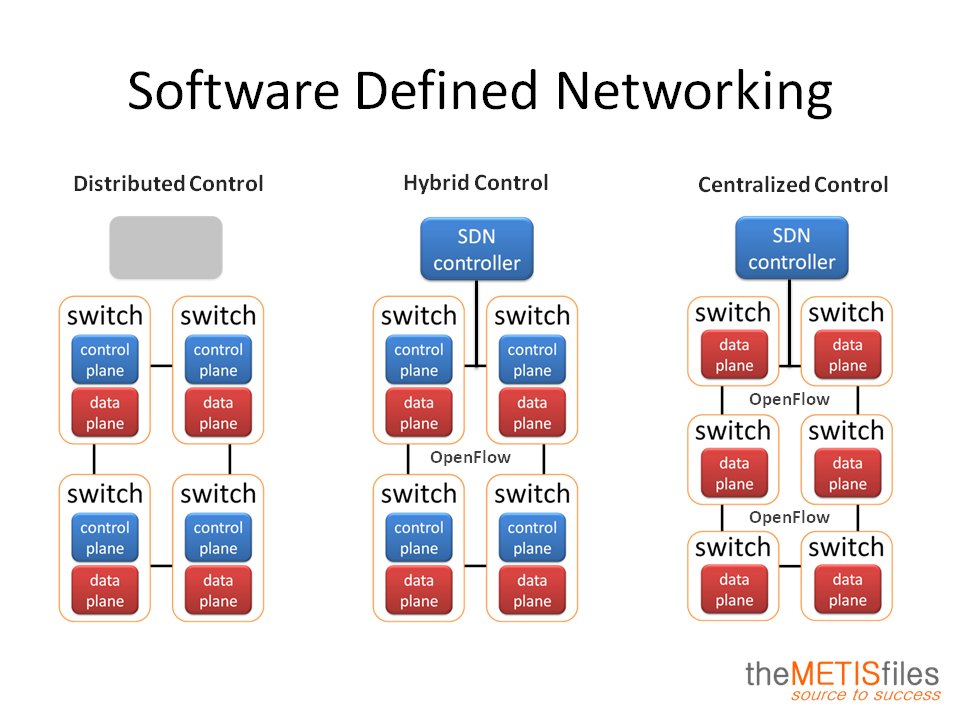
\includegraphics[scale=0.5]{./Drawings/ETSN10-Network_Architecture_Performance/software-defined-networking.png}
  \caption{Software Defined Networking \\ \href{https://www.themetisfiles.com/2012/10/the-future-of-the-network-is-software-defined/}{Source}}
  \label{fig:SDN}
\end{figure}

\paragraph{Network Function Virtualization}\label{par:NFV}
Network Function Virtualization is a massive part in why 5G is going to be able to scale to handle the traffic that will be placed on it.

\begin{definition}[Network Function Virtualization]\label{def:Network_Function_Virtualization}
  \emph{Network Function Virtualization} (\emph{NFV}) is the process of taking functions that used to be performed by dedicated physical entities and virtualizing them.
  This way, there are virtual machines or containers running the same functions as the physical hardware, but multiple instances can run on the same hardware.
  This also allows for dynamic scaling as the network demands.

  \begin{remark}[\nameref*{def:Software_Defined_Networking} Requirement]\label{rmk:NFV_Rely_SDN}
    \nameref{def:Network_Function_Virtualization} can only work because of \nameref{def:Software_Defined_Networking}.
    The only way to be able to move network functions around easily to have the funcctions be software-defined, allowing networks to reconfigure dynamically.
  \end{remark}

  \begin{remark}[Core 5G Functionality]\label{rmk:NFV_Core_5G}
    \nameref{def:Network_Function_Virtualization} is one of the 3 \textbf{MAJOR} functionalities that is enabling 5G to happen.
  \end{remark}
\end{definition}

\paragraph{Network Slicing}\label{par:Network_Slicing}
\begin{definition}[Network Slicing]\label{def:Network_Slicing}
  \emph{Network Slicing} is a network architecture that enables the multiplexing of virtualized and independent logical networks on the same physical network infrastructure.
  Each network slice is an isolated end-to-end network, thus it has its own Quality of Service requirements and management techniques.
  These slices can be tailored to fulfill diverse requirements as requested by a particular application.
  \begin{itemize}[noitemsep]
  \item A mobile broadband slice can handle Quality of Service for video streams.
  \item A URLLC slice can prioritize alarm packets.
  \end{itemize}

  \begin{remark}[Core 5G Functionality]\label{rmk:Network_Slicing_Core_5G}
    \nameref{def:Network_Slicing} is one of the 3 \textbf{MAJOR} functionalities that is enabling 5G to happen.
  \end{remark}
\end{definition}
\textbf{TODO!!}

\paragraph{Cloud RAN}\label{par:Cloud_RAN}
\begin{definition}[Cloud Radio Access Network]\label{def:Cloud_RAN}

\end{definition}
\textbf{TODO!!}

\paragraph{Frame Structure}\label{par:Frame_Structure}
\textbf{TODO!!}

\paragraph{Enabling Technologies for 5G}\label{par:5G_Enabling_Technologies}
\textbf{TODO!!}

\subparagraph{Millimeter Wave}\label{subpar:Millimeter_Wave}
\textbf{TODO!!}

\subparagraph{Small Cells}\label{subpar:Small_Cells}
\textbf{TODO!!}

\subparagraph{Massive MIMO}\label{subpar:Massive_MIMO}
\textbf{TODO!!}

%%% Local Variables:
%%% mode: latex
%%% TeX-master: "../../ETSN10-Network_Architecture_Performance-Reference_Sheet"
%%% End:


%%% Local Variables:
%%% mode: latex
%%% TeX-master: "../ETSN10-Network_Architecture_Performance-Reference_Sheet"
%%% End:
